\documentclass[fleqn]{beamer}

\usepackage[british]{babel}
\usepackage{graphicx,ru,url}
\usepackage{amsmath}
% Use Times for math font and text font.
\RequirePackage[T1]{fontenc}
%\RequirePackage{txfonts}
% bold math must be loaded after Times font
\usepackage{bm}
\usepackage{booktabs} % nice rules (thick lines) for tables
\usepackage{microtype} % improves typography for PDF
\usepackage{xcolor}
\usepackage{tikz}
\usepackage{verbatim}
\usetikzlibrary{arrows,shapes,snakes}
\usepackage{hyperref}

% The title of the presentation:
%  - first a short version which is visible at the bottom of each slide;
%  - second the full title shown on the title slide;
\title[Updating PWR Simulator]{
    Updating a PWR Simulator in Python}

% Optional: a subtitle to be displayed on the title slide
%\subtitle{Show where you're from}

% The author(s) of the presentation:
%  - again first a short version to be displayed at the bottom;
%  - next the full list of authors, which may include contact information;
\author[Reed, Hayhurst]{
    Richard Reed, Jacob Hayhurst, Shravan Gangadhara \\
    Dr. Jeremy Roberts}

% The institute:
%  - to start the name of the university as displayed on the top of each slide
%    this can be adjusted such that you can also create a Dutch version
%  - next the institute information as displayed on the title slide
\institute[Kansas State University]{
    Mechanical and Nuclear Engineering \\
    Kansas State University}

% Add a date and possibly the name of the event to the slides
%  - again first a short version to be shown at the bottom of each slide
%  - second the full date and event name for the title slide
\date[2016 Student Conference]{
    2016 ANS Student Conference \\
    April 2016}

\begin{document}
    %\renewcommand*{\inserttotalframenumber}{\pageref{lastframe}}
    \newcommand{\beginbackup}{
        \newcounter{framenumbervorappendix}
        \setcounter{framenumbervorappendix}{\value{framenumber}}
    }
    \newcommand{\backupend}{
        \addtocounter{framenumbervorappendix}{-\value{framenumber}}
        \addtocounter{framenumber}{\value{framenumbervorappendix}} 
    }
    
    \begin{frame}
        \titlepage
    \end{frame}
    
    \begin{frame}
        \frametitle{Outline}
        \begin{block}{Presentation Outline}
            \begin{itemize}
                \item Introduction and Background
                \begin{itemize}
                    \item Motivation and Goals
                    \item Original Fortran
                \end{itemize}
                \item Physical Models
                \item Graphical User Interface
                \item Conclusion
            \end{itemize}
        \end{block}
    \end{frame}
    
    \section{Introduction and Background}
    
    \begin{frame}
        \frametitle{Introduction and Background}
        \begin{block}{Motivation}
            \begin{itemize}
                \item PRISM only works on DOS
                \item PRISM is useful for teaching tool
                \item Python and Kivy are cross platform and modern languages
            \end{itemize}
        \end{block}
        \begin{block}{Goals}
            \begin{itemize}
                \item Translate Physical models from Fortran 77 to Python
                \item Recreate GUI using Kivy Library
                \item Validate the results against original PRISM
                \item Support cross-platform versions of program
            \end{itemize}
        \end{block}
    \end{frame}
    
    \begin{frame}
        \frametitle{Original Fortran}
        \begin{center}
            Screenshot of the Landing Page for DOS based GUI 
            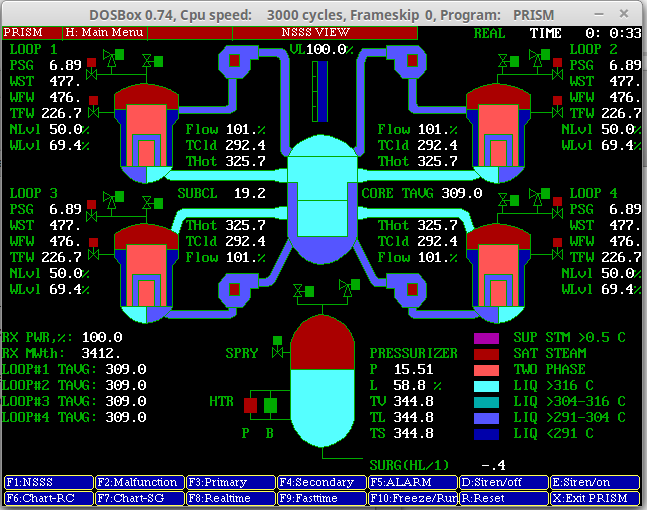
\includegraphics[trim=0cm 0cm 0cm .85cm, clip=true, totalheight=.8\textheight]{prism}
        \end{center}
    \end{frame}
    
    \begin{frame}
        \frametitle{Original Fortran}
        \begin{center}
            Screenshot of the Malfunction for DOS based GUI 
            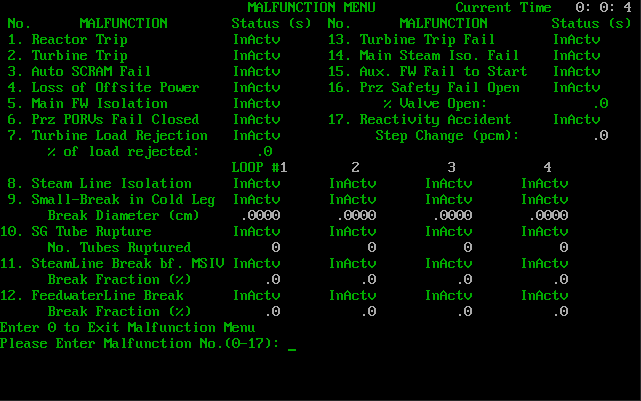
\includegraphics[totalheight=.8\textheight]{prism2}
        \end{center}
    \end{frame}
    
    \begin{frame}
        \frametitle{Original Fortran}
        \begin{center}
            Screenshot of the Primary Data Page for DOS based GUI 
            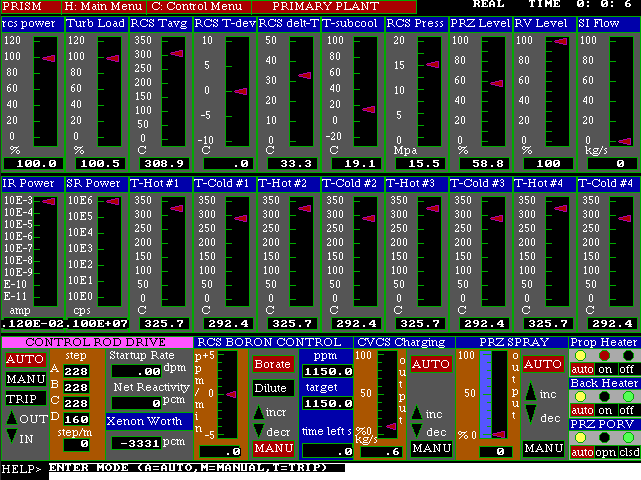
\includegraphics[totalheight=.8\textheight]{prism3}
        \end{center}
    \end{frame}
    
    \begin{frame}
        \frametitle{Original Fortran}
        \begin{center}
            Screenshot of the Secondary Data Page for DOS based GUI 
            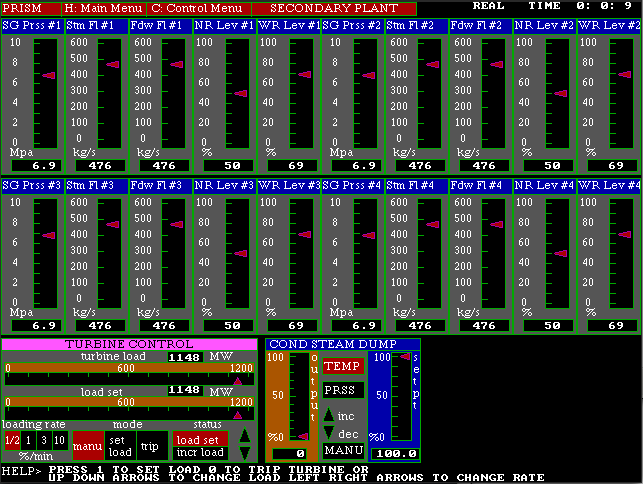
\includegraphics[totalheight=.8\textheight]{prism4}
        \end{center}
    \end{frame}
    
    \begin{frame}
        \frametitle{Original Fortran}
        \begin{center}
            Screenshot of the Alarm Panel for DOS based GUI 
            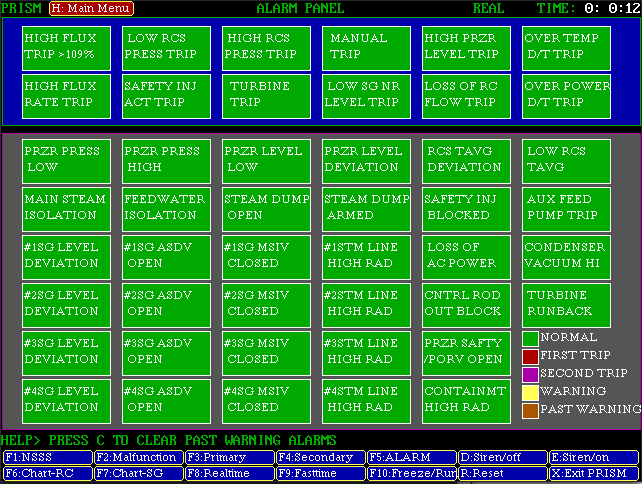
\includegraphics[totalheight=.8\textheight]{prism5}
        \end{center}
    \end{frame}
    
    \section{Physical Models}
    \begin{frame}
        \frametitle{PRISM Noding Scheme}
        \centering
        \begin{figure}
            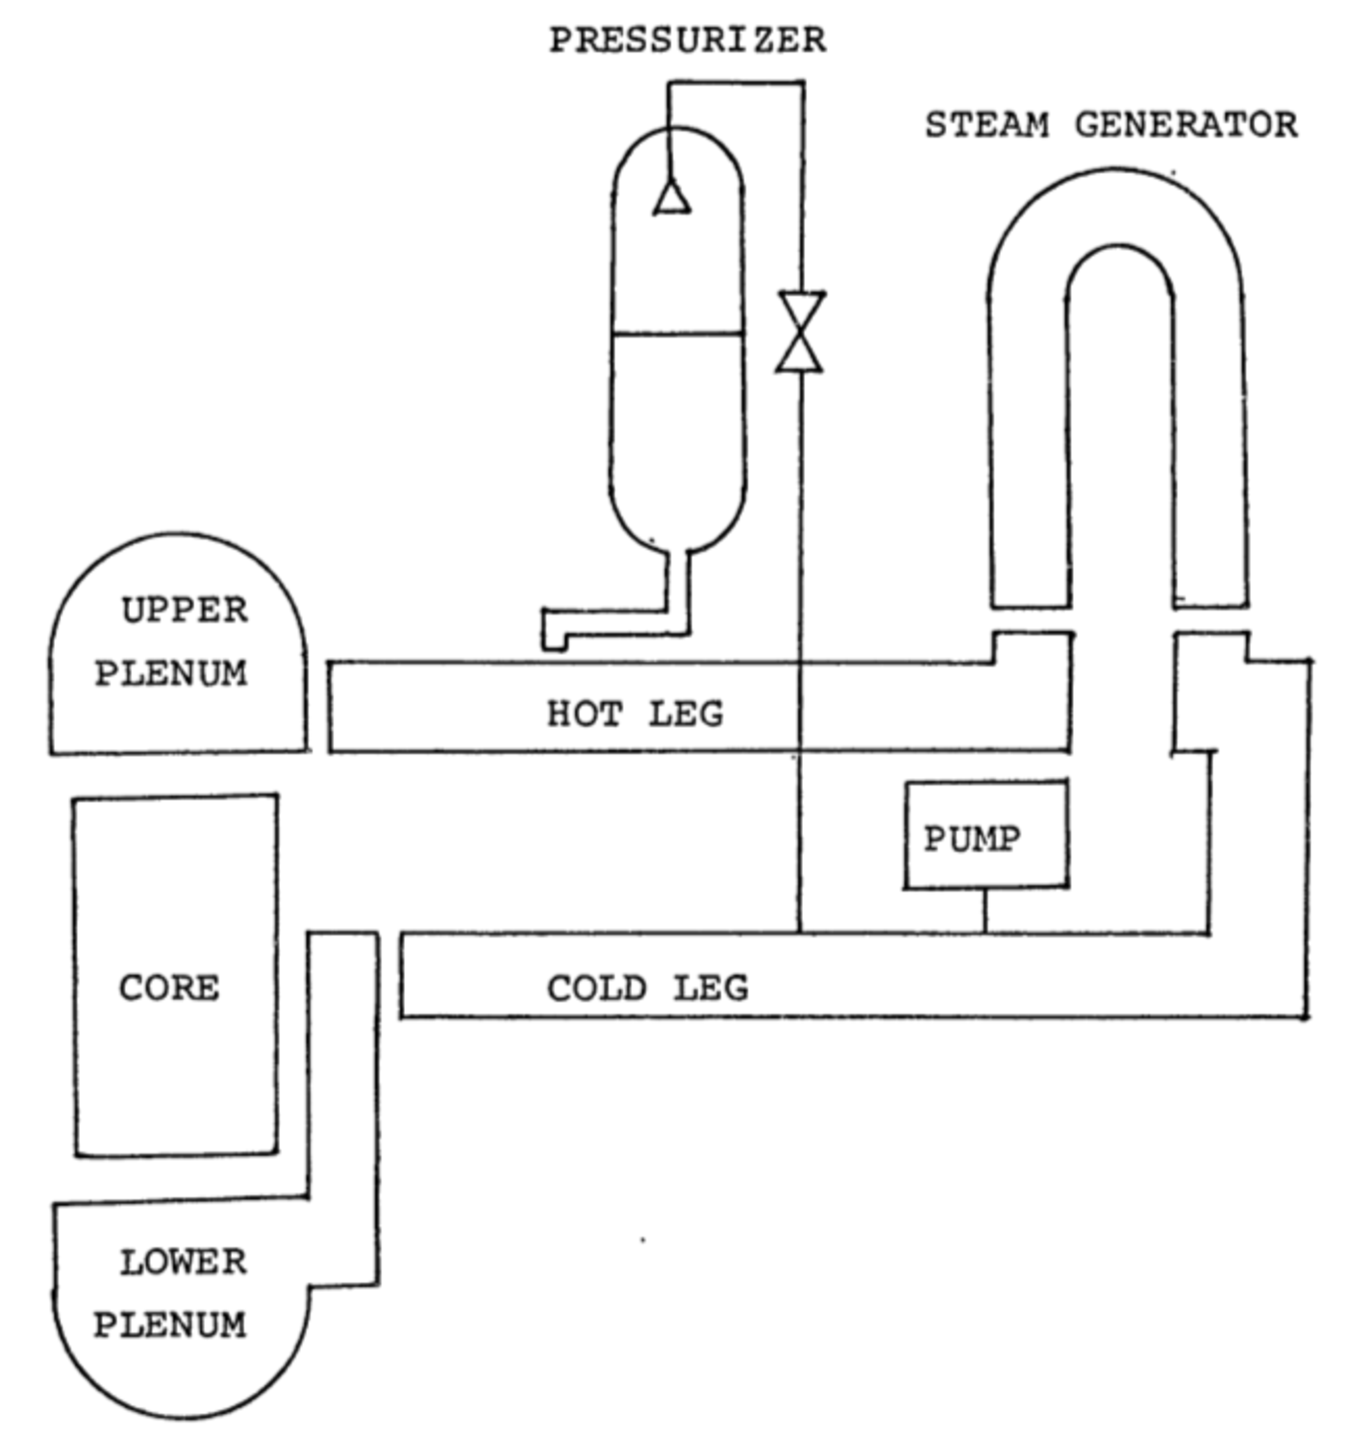
\includegraphics[totalheight=0.8\textheight]{prism_thesis.pdf}
        \end{figure}
    \end{frame}
    \begin{frame}
        \frametitle{Component Models}
        \centering
        \begin{block}{Core Model}
            \begin{itemize}
                \item Point kinetics model with 6 delayed groups
                \item Lumped-fuel heat transfer model
                \item Single Node Model
            \end{itemize}
        \end{block}
        \begin{block}{Pressurizer Model}
            \begin{itemize}
                \item Uniform properties in each phase
                \item No metastability in either phase
                \item Rainout prevents subcooling by maintaining sat vapor
                \item Flashing prevents superheating by maintaining sat liquid
                \item Spray enters the vessel as a sat liquid
                \item No heat is transfered at the liquid-vapor interface
            \end{itemize}
        \end{block}
    \end{frame}
    
    
    \section{Graphical User Interface}
    \begin{frame}
        \frametitle{Graphical User Interface}
        \begin{block}{Kivy Library}
            \begin{itemize}
                \item Created in February 2011
                \begin{itemize}
                    \item Matthew Virbel and others
                    \item French Programmer
                \end{itemize}
                \item Separates mechanics and graphics into two separate files
                \item Python library that uses the KV language
                \item Designed to port to all platforms and mobile devices
            \end{itemize}
        \end{block}
    \end{frame}
    
    \begin{frame}
        \frametitle{PRISM Redesigned}
        \begin{center}
            Updated landing page designed with Kivy
            \includegraphics[totalheight=.75\textheight]{PrismNew}
        \end{center}
    \end{frame}
    
    \section{Conclusion}
    \begin{frame}
        \frametitle{Conclusions}
        \begin{block}{Conclusions}
            \begin{itemize}
                \item DOS based PRISM is outdated
                \item Python and Kivy are used to update PRISM
                \item Program will be used as teaching tool primarily
                \item Nearly completed implementation
            \end{itemize}
        \end{block}
        \begin{columns}[T]
            \begin{column}{0.5\textwidth}
                \begin{block}{Future Work}
                    \begin{itemize}
                        \item Verification and Validation
                        \item Deploy on various platforms
                        \item Update physical models
                    \end{itemize}
                \end{block}
            \end{column}
            \begin{column}{0.5\textwidth}
                \begin{block}{Acknowledgements}
                    Kansas State Electrical Power Affiliates Program (EPAP)
                \end{block}
            \end{column}
        \end{columns}
        \nocite{*}
    \end{frame}
    
    \begin{frame}[t,allowframebreaks]\label{lastframe}
        \frametitle{References}
        \bibliographystyle{ans}
        \bibliography{bibliography}
    \end{frame}
    
%     \beginbackup
    
%     \begin{frame}[noframenumbering]
%         \frametitle{10-pin 238 g Library}
%     \end{frame}
    
%     \backupend
    
\end{document}
